\ifx\wholebook\relax\else

% --------------------------------------------
% Lulu:

    \documentclass[a4paper,12pt,twoside]{../includes/ThesisStyle}

	\usepackage[T1]{fontenc} %%%key to get copy and paste for the code!
%\usepackage[utf8]{inputenc} %%% to support copy and paste with accents for frnehc stuff
\usepackage{times}
\usepackage{ifthen}
\usepackage{xspace}
\usepackage{alltt}
\usepackage{latexsym}
\usepackage{url}            
\usepackage{amssymb}
\usepackage{amsfonts}
\usepackage{amsmath}
\usepackage{stmaryrd}
\usepackage{enumerate}
\usepackage{cite}
%\usepackage[pdftex,colorlinks=true,pdfstartview=FitV,linkcolor=blue,citecolor=blue,urlcolor=blue]{hyperref}
\usepackage{xspace}
%\usepackage{graphicx}
\usepackage{subfigure}
\usepackage[scaled=0.85]{helvet}
        
        
\newcommand{\sepe}{\mbox{>>}}
\newcommand{\pack}[1]{\emph{#1}}
\newcommand{\ozo}{\textsc{oZone}\xspace}
\newcommand\currentissues{\par\smallskip\textbf{Current Issues -- }}

\newboolean{showcomments}
\setboolean{showcomments}{true}
\ifthenelse{\boolean{showcomments}}
  {\newcommand{\bnote}[2]{
	\fbox{\bfseries\sffamily\scriptsize#1}
    {\sf\small$\blacktriangleright$\textit{#2}$\blacktriangleleft$}
    % \marginpar{\fbox{\bfseries\sffamily#1}}
   }
   \newcommand{\cvsversion}{\emph{\scriptsize$-$Id: macros.tex,v 1.1.1.1 2007/02/28 13:43:36 bergel Exp $-$}}
  }
  {\newcommand{\bnote}[2]{}
   \newcommand{\cvsversion}{}
  } 


\newcommand{\here}{\bnote{***}{CONTINUE HERE}}
\newcommand{\nb}[1]{\bnote{NB}{#1}}
\newcommand{\fix}[1]{\bnote{FIX}{#1}}
%%%% add your own macros 

\newcommand{\sd}[1]{\bnote{Stef}{#1}}
\newcommand{\ja}[1]{\bnote{Jannik}{#1}}
\newcommand{\na}[1]{\bnote{Nico}{#1}}
%%% 


\newcommand{\figref}[1]{Figure~\ref{fig:#1}}
\newcommand{\figlabel}[1]{\label{fig:#1}}
\newcommand{\tabref}[1]{Table~\ref{tab:#1}}
\newcommand{\layout}[1]{#1}
\newcommand{\commented}[1]{}
\newcommand{\secref}[1]{Section \ref{sec:#1}}
\newcommand{\seclabel}[1]{\label{sec:#1}}

%\newcommand{\ct}[1]{\textsf{#1}}
\newcommand{\stCode}[1]{\textsf{#1}}
\newcommand{\stMethod}[1]{\textsf{#1}}
\newcommand{\sep}{\texttt{>>}\xspace}
\newcommand{\stAssoc}{\texttt{->}\xspace}

\newcommand{\stBar}{$\mid$}
\newcommand{\stSelector}{$\gg$}
\newcommand{\ret}{\^{}}
\newcommand{\msup}{$>$}
%\newcommand{\ret}{$\uparrow$\xspace}

\newcommand{\myparagraph}[1]{\noindent\textbf{#1.}}
\newcommand{\eg}{\emph{e.g.,}\xspace}
\newcommand{\ie}{\emph{i.e.,}\xspace}
\newcommand{\ct}[1]{{\textsf{#1}}\xspace}


\newenvironment{code}
    {\begin{alltt}\sffamily}
    {\end{alltt}\normalsize}

\newcommand{\defaultScale}{0.55}
\newcommand{\pic}[3]{
   \begin{figure}[h]
   \begin{center}
   \includegraphics[scale=\defaultScale]{#1}
   \caption{#2}
   \label{#3}
   \end{center}
   \end{figure}
}

\newcommand{\twocolumnpic}[3]{
   \begin{figure*}[!ht]
   \begin{center}
   \includegraphics[scale=\defaultScale]{#1}
   \caption{#2}
   \label{#3}
   \end{center}
   \end{figure*}}

\newcommand{\infe}{$<$}
\newcommand{\supe}{$\rightarrow$\xspace}
\newcommand{\di}{$\gg$\xspace}
\newcommand{\adhoc}{\textit{ad-hoc}\xspace}

\usepackage{url}            
\makeatletter
\def\url@leostyle{%
  \@ifundefined{selectfont}{\def\UrlFont{\sf}}{\def\UrlFont{\small\sffamily}}}
\makeatother
% Now actually use the newly defined style.
\urlstyle{leo}



	\usepackage{amsmath,amssymb}             % AMS Math
% \usepackage[french]{babel}
\usepackage[latin1]{inputenc}
\usepackage[T1]{fontenc}
\usepackage[left=1.5in,right=1.3in,top=1.1in,bottom=1.1in,includefoot,includehead,headheight=13.6pt]{geometry}
\renewcommand{\baselinestretch}{1.05}

\usepackage{multicol}

% Table of contents for each chapter

\usepackage[nottoc, notlof, notlot]{tocbibind}
\usepackage{minitoc}
\setcounter{minitocdepth}{1}
\mtcindent=15pt
% Use \minitoc where to put a table of contents

\usepackage{enumitem}

\usepackage{aecompl}

% Glossary / list of abbreviations

%\usepackage[intoc]{nomencl}
%\renewcommand{\nomname}{List of Abbreviations}
%
%\makenomenclature

% My pdf code

\usepackage[pdftex]{graphicx}
\usepackage[a4paper,pagebackref,hyperindex=true]{hyperref}

\usepackage{pgfplotstable,booktabs,colortbl}
\pgfplotsset{compat=1.8}

% Links in pdf
\usepackage{color}
\definecolor{linkcol}{rgb}{0,0,0.4} 
\definecolor{citecol}{rgb}{0.5,0,0} 

% Change this to change the informations included in the pdf file

% See hyperref documentation for information on those parameters

\hypersetup
{
bookmarksopen=true,
pdftitle="Sista: a Metacircular Architecture for Runtime Optimisation Persistence",
pdfauthor="Clement BERA", 
pdfsubject="Thesis", %subject of the document
%pdftoolbar=false, % toolbar hidden
pdfmenubar=true, %menubar shown
pdfhighlight=/O, %effect of clicking on a link
colorlinks=true, %couleurs sur les liens hypertextes
pdfpagemode=None, %aucun mode de page
pdfpagelayout=SinglePage, %ouverture en simple page
pdffitwindow=true, %pages ouvertes entierement dans toute la fenetre
linkcolor=linkcol, %couleur des liens hypertextes internes
citecolor=citecol, %couleur des liens pour les citations
urlcolor=linkcol %couleur des liens pour les url
}

% definitions.
% -------------------

\setcounter{secnumdepth}{3}
\setcounter{tocdepth}{1}

% Some useful commands and shortcut for maths:  partial derivative and stuff

\newcommand{\pd}[2]{\frac{\partial #1}{\partial #2}}
\def\abs{\operatorname{abs}}
\def\argmax{\operatornamewithlimits{arg\,max}}
\def\argmin{\operatornamewithlimits{arg\,min}}
\def\diag{\operatorname{Diag}}
\newcommand{\eqRef}[1]{(\ref{#1})}

\usepackage{rotating}                    % Sideways of figures & tables
%\usepackage{bibunits}
%\usepackage[sectionbib]{chapterbib}          % Cross-reference package (Natural BiB)
%\usepackage{natbib}                  % Put References at the end of each chapter
                                         % Do not put 'sectionbib' option here.
                                         % Sectionbib option in 'natbib' will do.
\usepackage{fancyhdr}                    % Fancy Header and Footer

% \usepackage{txfonts}                     % Public Times New Roman text & math font
  
%%% Fancy Header %%%%%%%%%%%%%%%%%%%%%%%%%%%%%%%%%%%%%%%%%%%%%%%%%%%%%%%%%%%%%%%%%%
% Fancy Header Style Options

\pagestyle{fancy}                       % Sets fancy header and footer
\fancyfoot{}                            % Delete current footer settings

%\renewcommand{\chaptermark}[1]{         % Lower Case Chapter marker style
%  \markboth{\chaptername\ \thechapter.\ #1}}{}} %

%\renewcommand{\sectionmark}[1]{         % Lower case Section marker style
%  \markright{\thesection.\ #1}}         %

\fancyhead[LE,RO]{\bfseries\thepage}    % Page number (boldface) in left on even
% pages and right on odd pages
\fancyhead[RE]{\bfseries\nouppercase{\leftmark}}      % Chapter in the right on even pages
\fancyhead[LO]{\bfseries\nouppercase{\rightmark}}     % Section in the left on odd pages

\let\headruleORIG\headrule
\renewcommand{\headrule}{\color{black} \headruleORIG}
\renewcommand{\headrulewidth}{1.0pt}
\usepackage{colortbl}
\arrayrulecolor{black}

\fancypagestyle{plain}{
  \fancyhead{}
  \fancyfoot{}
  \renewcommand{\headrulewidth}{0pt}
}

\usepackage{algorithm}
\usepackage[noend]{algorithmic}

%%% Clear Header %%%%%%%%%%%%%%%%%%%%%%%%%%%%%%%%%%%%%%%%%%%%%%%%%%%%%%%%%%%%%%%%%%
% Clear Header Style on the Last Empty Odd pages
\makeatletter

\def\cleardoublepage{\clearpage\if@twoside \ifodd\c@page\else%
  \hbox{}%
  \thispagestyle{empty}%              % Empty header styles
  \newpage%
  \if@twocolumn\hbox{}\newpage\fi\fi\fi}

\makeatother
 
%%%%%%%%%%%%%%%%%%%%%%%%%%%%%%%%%%%%%%%%%%%%%%%%%%%%%%%%%%%%%%%%%%%%%%%%%%%%%%% 
% Prints your review date and 'Draft Version' (From Josullvn, CS, CMU)
\newcommand{\reviewtimetoday}[2]{\special{!userdict begin
    /bop-hook{gsave 20 710 translate 45 rotate 0.8 setgray
      /Times-Roman findfont 12 scalefont setfont 0 0   moveto (#1) show
      0 -12 moveto (#2) show grestore}def end}}
% You can turn on or off this option.
% \reviewtimetoday{\today}{Draft Version}
%%%%%%%%%%%%%%%%%%%%%%%%%%%%%%%%%%%%%%%%%%%%%%%%%%%%%%%%%%%%%%%%%%%%%%%%%%%%%%% 

\newenvironment{maxime}[1]
{
\vspace*{0cm}
\hfill
\begin{minipage}{0.5\textwidth}%
%\rule[0.5ex]{\textwidth}{0.1mm}\\%
\hrulefill $\:$ {\bf #1}\\
%\vspace*{-0.25cm}
\it 
}%
{%

\hrulefill
\vspace*{0.5cm}%
\end{minipage}
}

\let\minitocORIG\minitoc
\renewcommand{\minitoc}{\minitocORIG \vspace{1.5em}}

\usepackage{multirow}
\usepackage{slashbox}

\newenvironment{bulletList}%
{ \begin{list}%
	{$\bullet$}%
	{\setlength{\labelwidth}{25pt}%
	 \setlength{\leftmargin}{30pt}%
	 \setlength{\itemsep}{\parsep}}}%
{ \end{list} }

\newtheorem{definition}{D�finition}
\renewcommand{\epsilon}{\varepsilon}

% centered page environment

\newenvironment{vcenterpage}
{\newpage\vspace*{\fill}\thispagestyle{empty}\renewcommand{\headrulewidth}{0pt}}
{\vspace*{\fill}}



	\graphicspath{{.}{../figures/}}
	\begin{document}
\fi

\chapter{State of the art}
\label{chap:stateOfTheArt}
\minitoc

%Overall intro + arch
The thesis is an attempt to build an optimising JIT for Pharo. We discuss in the first section about the two main different architectures possible to build an optimising JIT. The traditional architecture focuses on the optimisation of frequently used functions based on its previous runs. The modern architecture, the meta-tracing JITs, attempts to optimise linear sequences of frequently used instructions. The chapter follows by analysing existing work on the three reseach problems.

%metacircular
Firstly, the JITs written in a high-level language are discussed. Multiple high-level languages were used with different execution models. In the case where the optimising JIT is running in the same runtime than the optimised application, some JITs are able to optimise their own code. However, certains constraints exist to avoid metacircular issues.

%persistance
Secondly, most modern VMs always start-up an application with only non optimised code. This can be a problem in specific cases. For example, the application needs a certain amount of time, called \emph{warm-up time}, to reach peak performance, which is a problem if the application needs high-performance immediately. We detail how some VMs attempt to persist part of the optimisations across multiple start-ups.

%interface
Thirdly, the Sista architecture is designed so that the optimising JIT re-use the baseline JIT as a back-end while being written in a different programming language. We detail one of the rare cases where the JIT back-end is shared between the baseline JIT and the optimising JIT. We follow up by discussing the interface provided from the VM to generate and execute efficient machine code.

%what do we discuss
The chapter tries to discuss the main production and research open source VMs. Specific closed-source VMs are described because they are relevant in the context the thesis. However, most closed-source VMs are ignored as it is too difficult to get reliable information about them. 

%Smalltalk.
Commercial Smalltalk VMs existing today are closed-source and do not feature optimising JITs so we do not discuss them. In the 90s, the Self VM (CITE) and the Strongtalk VM (CITE) were able to execute Smalltalk code using an optimising JIT. Those VMs are briefly discussed but as far as we know there are not used in production today and no further development on those VMs is in progress.

%%%%%%%%%%%%%%%%%%%%%%%%%%%%%%%%%%%%%%%%%%%%%%%%%%%%%%%%%%%%%%%%%%%%%%%%%%%%%%%%%%%%%%%%%%%%%%%%%%%%%%%%%%%%%%%%%%%%%%%%%%%%%%%%%%%%%%%%%%%%%%%%%%%%%%%%%%%%%%%%%%%%%%%

\section{Optimising Just-in-Time compiler architectures}

Standard object-oriented languages feature dynamic dispatch. This is typically done through the use of virtual calls: the function to activate for each virtual call depends on information available at runtime but not at compile-time. Because of dynamic dispatch, it is difficult for an ahead-of-time compiler to optimise efficiently the code to execute. This problem is very important for languages such as Smalltalk where every call is a virtual call.

To avoid the problem, one solution is to use a JIT. The first runs of a function are done through a slow path, such as an interpreter or through a baseline JIT. Statistics are collected from these first runs to direct optimisations such as what functions each virtual call has activated. 

Two main architecture are present in modern VMs. On the one hand, the traditional approach compiles and optimises frequently used functions. On the other hand, the meta-tracing JITs optimise a linear sequence of frequently used instructions.

\subsection{Traditionnal architecture}

The traditionnal optimising JIT architecture is composed of multiple tiers. Each tier requires more time than the previous tier to compile the function to execute but the generated code is more efficient than the previous tier. 

In most VMs following this architecture, three tiers are present:
\begin{enumerate}
	\item \emph{Tier 1: v-function interpreter: } The first tier is a virtual function interpreter. In most VMs, no compilation time is required at all to interpret a v-function~\footnote{Some VMs require compilation time for interpretation because the v-functions are not provided in an executable format (for example source code is provided instead).}. However, the execution by the interpreter is not very fast.
	\item \emph{Tier 2: baseline JIT: } The second tier is the baseline JIT, which generates from the v-function a n-function with a limited number of optimisations. Once compiled, the n-function is used to execute the function instead of interpreting the v-function. A small amount of time is wasted to generate the n-function and the execution of the n-function is faster than interpreting the v-function. Baseline JITs usually generates inline caches (CITE): each virtual call has a local cache with the functions it has activated, both speeding-up the execution and collecting runtime information for the next tier.
	\item \emph{Tier 3: optimising JIT: } The last tier is the optimising JIT, which generates an optimised n-function. The optimising JIT uses runtime information such as the inline cache data to speculate on what function is called at each virtual calls, allowing to perform inlining and generating the optimised n-function from multiple v-functions. Such optimisations greatly speed-up execution but are invalid if one of the compile-time speculation is not valid at runtime. In this case, the VM deoptimises the code and re-optimise it differently. The optimising JIT require more time than the baseline JIT to generate n-functions, but the generated code is much faster.
\end{enumerate}

\begin{figure}[h!]
    \begin{center}
        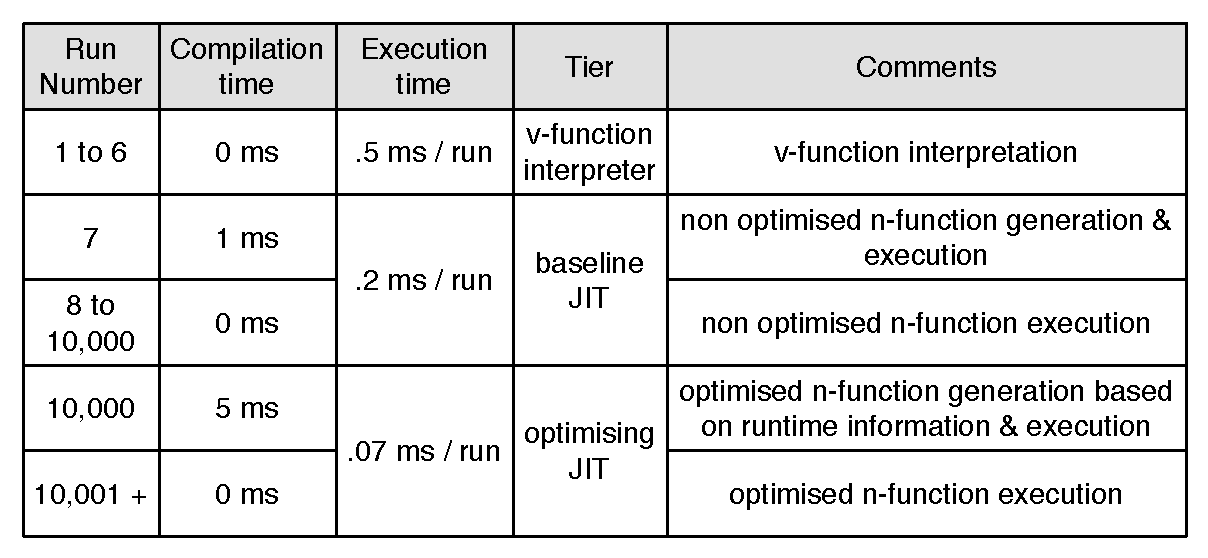
\includegraphics[width=0.95\linewidth]{TieredArchitecture}
        \caption{Execution of a frequently used v-function}
        \label{fig:TieredArchitecture}
    \end{center}
\end{figure}

Figure \ref{fig:TieredArchitecture} shows the execution of a frequently used v-functions over the three tiers. The first few runs are interpreted, each run taking 0.5 ms. The following run requires some compilation time for the baseline JIT to kick in, but the function is then executed 2.5 times faster and runtime information is collected. Lastly, after 10,000 runs, the optimising JIT takes a significant amount of time to generate an optimised n-function, but the optimised version is three times faster than the baseline JIT version.


The first VM featuring this traditional tiered architecture was the Self VM (CITE). The Self VM had only two tiers, the baseline JIT and the optimising JIT, which they called "the non optimising compiler" and "the optimising compiler". The Self programming language has never really become popular so the VM is not really used anymore. 

The second VM built with this design was the animorphic VM for the Strongtalk programming language(CITE), a Smalltalk dialect. This VM is the first to feature three tiers. The first tier is a threaded code interpreter hence interpretation requires a small amount of compilation time to generate threaded code from the v-function. The two other tiers are the same as in the Self-VM. The animorphic VM has never reached production.

Then the hotspot VM (CITE) was implemented, which has been the default Java VM provided by Oracle for more than a decade. More recently, the V8 Javascript engine (CITE), used for Google Chrome and Node JS and the Dart VMs are built using similar architectures.  

\paragraph{Number of tiers.} Most featuring this design have three tiers. The number of tiers can however vary from two to four. The following paragraphs discuss the reasons why the VM implementors may choose to more or less tiers.

Each new tier needs to be maintained and evolved accordingly to the other tiers. Hence, a VM having more tiers requires more engineering time for maintainance and evolutions as any bug can come from any tier and evolutions need to be implemented on each tier. To lower the VM maintenance and evolution cost, a VM needs to have the least number of tiers possible.

By design, the optimising JIT is the key component for high-performance and it needs runtime information from previous runs to generate optimised code. Hence, a VM with the tiered architecture requires at least two tiers. One tier is used for the first runs to collect statistical information and the second tier generates optimised code. 

It is currently not possible to collect runtime information without overhead from a virtual function interpreter if the interpreter is written in a machine independent language. However, the inline cache technique allows to collect such information while speeding-up code execution over a v-function interpreter. Hence, using a v-function interpreter to collect runtime information is much slower than using a baseline JIT. For this reason, a VM with two tiers is most likely going to be designed with a baseline JIT and an optimising JIT. The Self VM was done exactly like that and the V8 Javascript engine was running this way from 2008 to 2016.

The interpreter tier is present in most VMs for two main reasons. Firstly, v-functions are usually more compact than n-functions. Being able to interpret v-functions allow to always keep functions rarely executed in v-function representation, lowering the memory footprint. Secondly, starting-up an application usually require the execution of multiple functions once to initialize the application. If a function is executed only once, the interpreter is usually faster because the compilation time is not worth it for one run. If we take the example in figure \ref{fig:TieredArchitecture}, we see that interpreting the v-function once takes 0.5 ms while compiling it with the baseline JIT and executing it takes 1.2 ms. Not having an interpreter can lead to poor start-up performance. The V8 Javascript engine added an interpreter tier in 2016 for these purposes.

In general, the non optimising tiers (the v-function interpreter and the baseline JIT) are kept as simple as possible to ease maintainance and evolutions. Only the third tier, the optimising JIT, is complex to be able to generate efficient n-functions.

Adding more than three tiers is usually not worth it as it would mean additional maintenance and evolution cost. However, in specific languages such as Javascript the start-up performance is very important and it can be worth it to have two optimising JIT tiers to increase start-up performance. The Javascript Webkit VM has four tiers since 2015 (CITE). In this case, the VM team introduced two optimising JIT tiers after the interpreter and baseline JIT. One optimising JIT tier has smaller compilation time than the other one but produce less efficient n-function.

\paragraph{Sharing portion of compilers.}

Shared back-end in webkit 

Shared backend in TurboFan and WebAssembly

\paragraph{Native threads and optimising JITs}

opt in other native threads.

\paragraph{The Graal optimising JIT}

Designed to be plugged in other VMS ? Extracted from Maxine and put on hotspot. Can be used as a specific compiler.
Explain quickly multilanguage
Discuss Graal, Truffle + Graal.

describe the runtime model with threads here. Or somewhere else but we need thread description.

explain JIT generation from annotation on AST interpreter

\subsection{Meta-tracing architecture}

+ Mozilla monkeys
LuaJIT

Alternative for multi language
Rpython + Pypy.
RPython tool chain \cite{Rigo06a}

explain quickly metatracing from interpreter

present them here so they can be compared to later.

%%%%%%%%%%%%%%%%%%%%%%%%%%%%%%%%%%%%%%%%%%%%%%%%%%%%%%%%%%%%%%%%%%%%%%%%%%%%%%%%%%%%%%%%%%%%%%%%%%%%%%%%%%%%%%%%%%%%%%%%%%%%%%%%%%%%%%%%%%%%%%%%%%%%%%%%%%%%%%%%%%%%%%%

\section{Virtual machine implementation language}

Can the JIT optimise itself ?

\subsection{Low-level languages}

typically C / C++ or other

why advantages and cons

\subsection{High-level language compiled ahead-of-time}

2) DSl / HIGH level language compiling AOT to assembly code.

fig.


\subsection{High-level language}

3) Metacircular VM (check metacircular related work)

+ Truffle. HL language but not the same.

Say 2 sentence Bee Smalltalk, closed source but maybe open source later.

%%%%%%%%%%%%%%%%%%%%%%%%%%%%%%%%%%%%%%%%%%%%%%%%%%%%%%%%%%%%%%%%%%%%%%%%%%%%%%%%%%%%%%%%%%%%%%%%%%%%%%%%%%%%%%%%%%%%%%%%%%%%%%%%%%%%%%%%%%%%%%%%%%%%%%%%%%%%%%%%%%%%%%%

\section{Runtime state persistance}

Check paper Sista persistance

\subsection{Warm-up time}

1) Fast warm-up

Discuss tiered arch and lower warm-up.

saving metadata + strongtalk and maybe Dart

save machine code and Azul

AOT

\subsection{Snapshots}

2) Preheating through snapshot in Dart

Snapshot in general for Kernel ?

%%%%%%%%%%%%%%%%%%%%%%%%%%%%%%%%%%%%%%%%%%%%%%%%%%%%%%%%%%%%%%%%%%%%%%%%%%%%%%%%%%%%%%%%%%%%%%%%%%%%%%%%%%%%%%%%%%%%%%%%%%%%%%%%%%%%%%%%%%%%%%%%%%%%%%%%%%%%%%%%%%%%%%%

\section{Virtual machine interface}

\subsection{The Graal-Hotspot architecture}

+ Graal and interface

\subsection{WebAssembly}

WebAssembly 

%%%%%%%%%%%%%%%%%%%%%%%%%%%%%%%%%%%%%%%%%%%%%%%%%%%%%%%%%%%%%%%%%%%%%%%%%%%%%%%%%%%%%%%%%%%%%%%%%%%%%%%%%%%%%%%%%%%%%%%%%%%%%%%%%%%%%%%%%%%%%%%%%%%%%%%%%%%%%%%%%%%%%%%

%MAybe conclusion, 1 sentence what we did and what comes next

%%%%%%%%%%%%%%%%%%%%%%%%%%%%%%%%%%%%%%%%%%%%%%%%%%%%%%%%%%%%%%%%%%%%%%%%%%%%%%%%%%%%%%%%%%%%%%%%%%%%%%%%%%%%%%%%%%%%%%%%%%%%%%%%%%%%%%%%%%%%%%%%%%%%%%%%%%%%%%%%%%%%%%%

%FOLLOWING IS OLD VERSION FOR HISTORY.

%In this chapter, the most popular production VMs and relevant research VMs are discussed. In further chapter, the thesis' proposed architecture will be compared against those VMs. 

%Most popular production VMs, such as Java hotspot (Cite) or Javascript's V8 (Cite) VMs are written in C++. Using C++ as a performance oriented low-level programming language proved to be very effective as it is possible to write code in a performance oriented fashion. A clear separation is made between the VM and the programming language run so there are no metacircular problems.

%Most of those VMs start-up from the language kernel, a set of core librairies and either source files or files containing bytecodes. Reaching peak performance takes a certain amount of time as the VM needs to detect and optimise correctly frequently used patterns of code. Reportedly, this warm-up time can be from several milliseconds up to multiple days. To solve partially the warm-up problem, such VMs are built with a tiered-architecture: the first few executions are run slowly but without any compilation time, subsequent hundreds of executing are run a bit faster with limited compilation time while further execution are run at peak performance after a certain amount of compilation time.

%An interesting point ot note is that several mainstream VMs were led by the same person (Lars Bak), who became very good at implementing very efficient and easy-to-maintain VMs in C++ as he implemented multiple of those in his life. His work therefore pushed the direction of VM implementation in the C++ direction.

%Among the C++ virtual machines, we will detail two specific VMs have uncommon features that are relevant in the context of the thesis. 

%\subsection{Azul}
%The Azul VM \cite{Azul} is a closed-source VM and expensive VM for Java. As for all closed-source projects, no one external to the project can be certain of what the code is doing. However, word has been that the Azul VM is able to persist optimised machine code across multiple start-ups. If the application is started on another processor, then the saved machine code is simply discarded. 

%\subsection{Dart}
%The Dart VM is an open-source VM for the Dart programming language. Dart features snapshots for fast application start-up. In Dart, the programmer can generate different kind of snapshots \cite{Anna13a}. Since that publication, the Dart team have added two new kind of snapshots, specialized for iOS and Android application deployment, which are quite similar to our snapshots.


%As the sista architecture is implemented in the context of Smalltalk, it could be relevant to discuss existing Smalltalk virtual machines. These VMs are interesting for multiple reasons, but unfortunately many of the Smalltalk virtual machines in production today are closed-source, making the discussion around them not that relevant as information is missing and unaccessible. In addition, as far as we know, there are no production Smalltalk VM today with an optimising JIT compiler, so the comparison with such VMs is even less relevant. 

%However, speculative optimisations in VMs started with the Self VM (CITE), with Self being a Smalltalk-like language, and was followed up with the strongtalk VM (CITE). Both VMs are open-source and available today but none of them are used in production. Self had never really broken through mainstream programming while strongtalk had never reached production state.

\ifx\wholebook\relax\else
    \end{document}
\fi